\documentclass[11pt,compress]{beamer}
% deactivate beamer navigation
%\setbeamertemplate{navigation symbols}{}
%\usepackage{geometry}
%\geometry{papersize={180mm, 135mm}, top=-1.5mm} % 210mm, 297mm
\usepackage{../style/lmu-lecture}
\setbeamertemplate{frametitle}{\expandafter\uppercase\expandafter\insertframetitle}
%\useoutertheme{metropolis}
% remove section slides
\AtBeginSection[]
{
  \begin{frame}<beamer>
    \frametitle{Introduction to Machine Learning}
    \tableofcontents[currentsection]
  \end{frame}
}
% includepdf slides, pagecommad will set counter for framenumber
\usepackage{pdfpages}
\includepdfset{trim=0mm 0mm 0mm 0mm, pagecommand={\global\setcounter{framenumber}{\value{page}}}}
% trim=0mm 6mm 0mm 0mm, offset=0 15,
% add footer:
\usepackage{framed, color}
\usepackage{xcolor}
%\iffalse
\setbeamertemplate{footline}[text line]{%
    \noindent\hspace*{\dimexpr-\oddsidemargin-1in\relax}%
     \colorbox{white}{
     \makebox[\dimexpr\paperwidth-2\fboxsep\relax]{
     \color{black}
     \begin{minipage}[c][4.5ex][c]{0.5\linewidth}
       \secname
     \end{minipage}
     \hfill\begin{minipage}[c][4.5ex][c]{0.5\linewidth}
       \flushright
       \insertframenumber{}~/~\inserttotalframenumber~~
     \end{minipage}
     }}%
  \hspace*{-\paperwidth}
}
%\fi
\begin{document}
\setbeamercolor{background canvas}{bg=}

% General remark: hyperlinks in included pdfs are not clickable anymore in the combined pdf

% Include tuning lecture slides
\section{Tuning}
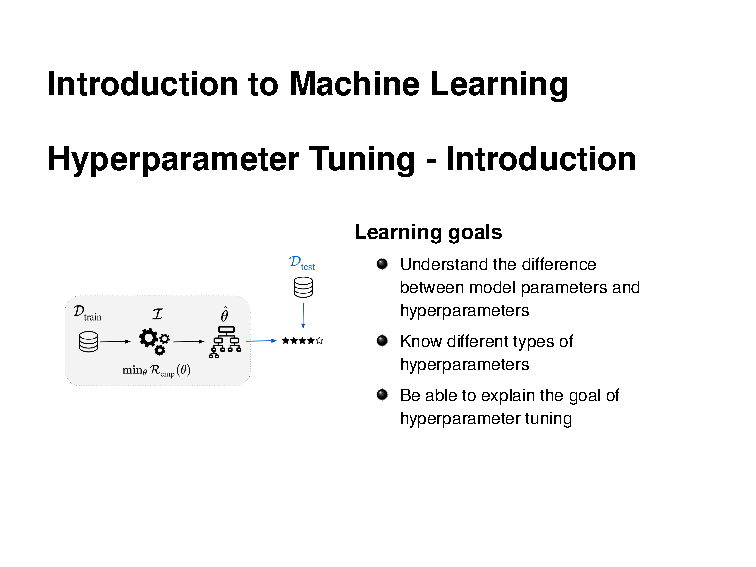
\includepdf[pages={1}, trim=0mm 0mm 0mm 40mm]{slides-tuning-intro.pdf} % remove title if you want
\includepdf[pages={2-last}]{slides-tuning-intro.pdf}
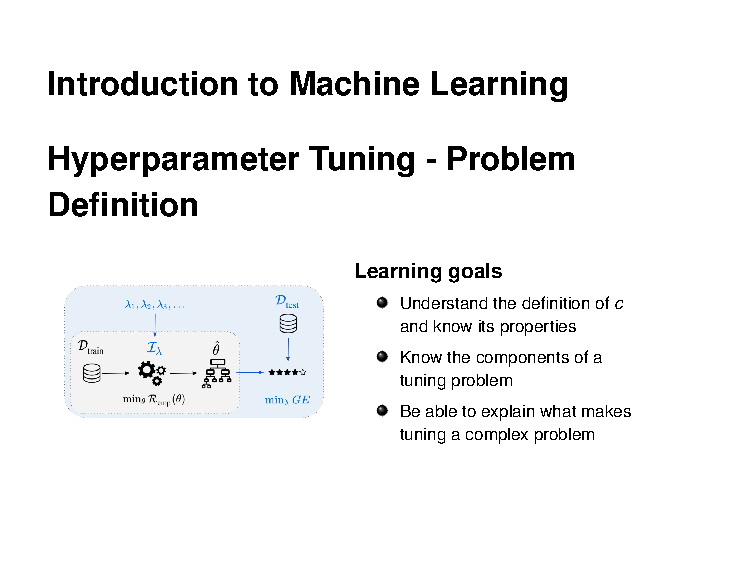
\includepdf[pages={1}, trim=0mm 0mm 0mm 40mm]{slides-tuning-tuningproblem.pdf}
\includepdf[pages={2-last}]{slides-tuning-tuningproblem.pdf}
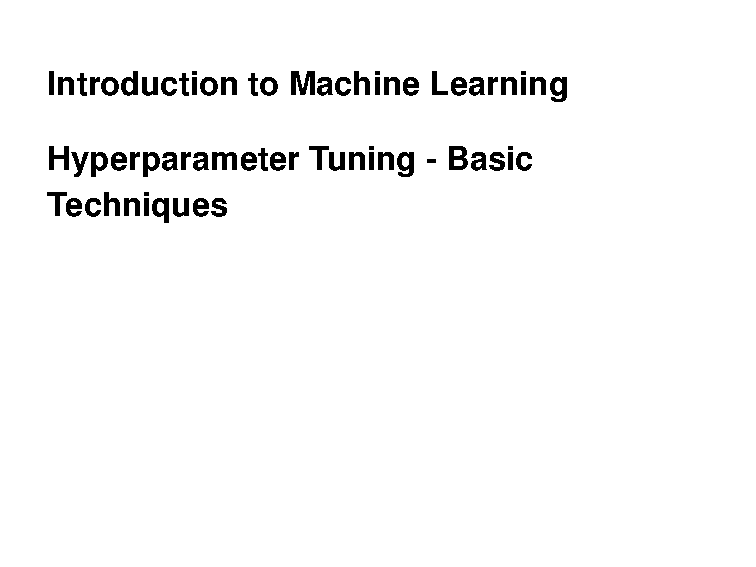
\includepdf[pages={1}, trim=0mm 0mm 0mm 40mm]{slides-tuning-basicalgos.pdf}
\includepdf[pages={2-last}]{slides-tuning-basicalgos.pdf}

% Include mlr3tuning lectures
\section{Tuning with mlr3}

\includepdf[pages={1-2, 6-8, 12-19, 23-35, 38-40, 43-53, 57, 62-69}]{../slides/mlr3/slides-mlr3-tuning.pdf}

% Add custom slide in between
\begin{frame}{Use Case Demo \& Exercise}
\begin{itemize}
\item \textbf{Demo:} \newline\href{https://mlr3gallery.mlr-org.com/posts/2020-03-11-mlr3tuning-tutorial-german-credit/}{\underline{mlr3tuning Tutorial}} (Excluding Section Nested Resampling)
\item \textbf{Exercise:}
\begin{enumerate}
\item Tune a decision tree (\texttt{rpart}) and specify the search space for \texttt{minsplit} (from 1 to 200) and \texttt{maxdepth} (from 10 to 30). Use 50 evaluations as termination criterion, the classification error \texttt{msr("classif.ce")} as performance measure, and 3-fold CV as resampling strategy.
\item Visualize the results using ggplot to see how \texttt{minsplit} and \texttt{maxdepth} affect the performance.
\item Optional: Change your previous code and use the brier score \texttt{msr("classif.bbrier")} as performance measure instead of the classification error for tuning (hint: You need to modify your learner such that it predicts probabilites).
\end{enumerate}
\end{itemize}
\end{frame}

% Include nested resampling lecture slides
\section{Nested Resampling}
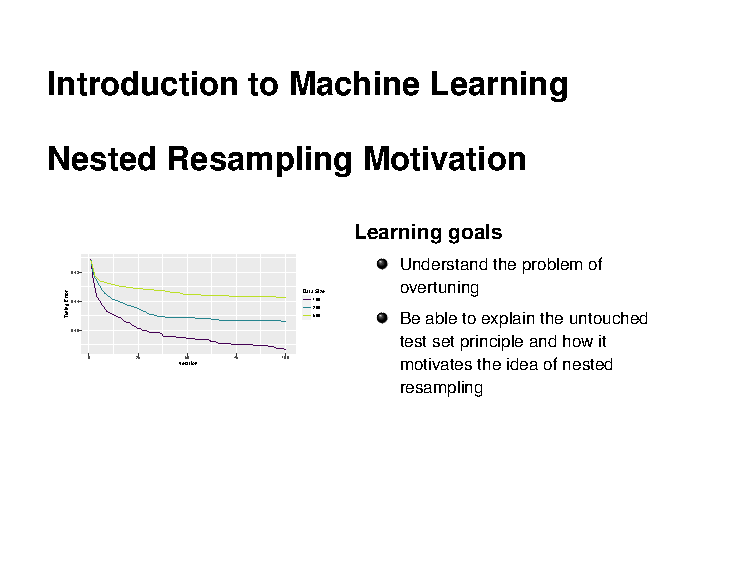
\includepdf[pages={1}, trim=0mm 0mm 0mm 40mm]{slides-nested-nestedintro.pdf}
\includepdf[pages={2-last}]{slides-nested-nestedintro.pdf}

\includepdf[pages={1}, trim=0mm 0mm 0mm 40mm]{slides-nested-trainvalidtest.pdf}

\includepdf[pages={2-last}]{slides-nested-trainvalidtest.pdf}
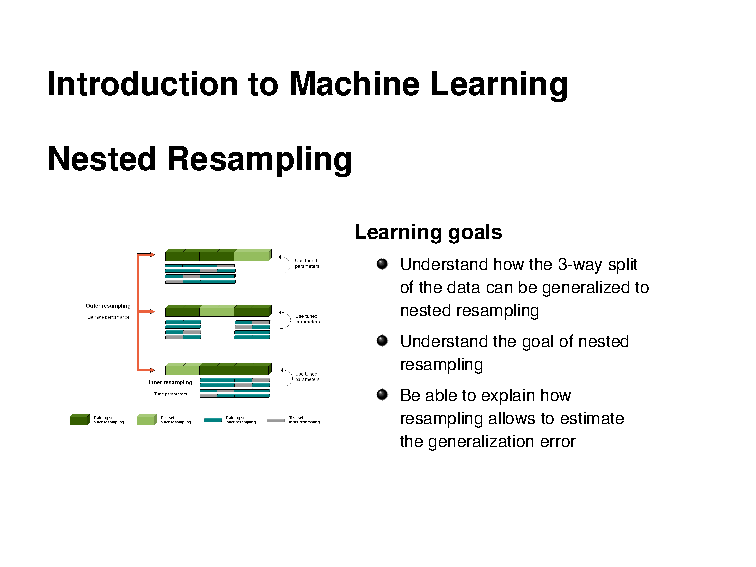
\includepdf[pages={1}, trim=0mm 0mm 0mm 40mm]{slides-nested-nestedresampling.pdf}
\includepdf[pages={2-last}]{slides-nested-nestedresampling.pdf}

% Add custom slide in between
\section{Nested Resampling with mlr3}

\includepdf[pages={70-last}]{../slides/mlr3/slides-mlr3-tuning.pdf}
\begin{frame}{Use Case Demo \& Exercise}
\begin{itemize}
\item \textbf{Demo:} \href{https://mlr3gallery.mlr-org.com/posts/2020-03-11-mlr3tuning-tutorial-german-credit/\#nested-resampling}{\underline{mlr3tuning Tutorial}} (Section Nested Resampling)
\item \textbf{Exercise:}
\begin{enumerate}
\item Create an \texttt{AutoTuner} based on a random forest (\texttt{ranger}), which automatically finds the best hyperparameters for \texttt{mtry} and \texttt{replace} based on random search.
See \texttt{?ranger} for a description of the parameters and use a meaningful number of evaluations and a meaningful search space.
\item Use the \texttt{benchmark} function to compare the performance of the \texttt{AutoTuner} against an untuned \texttt{ranger} and \texttt{rpart} learner in their default hyperparameter values.
\end{enumerate}
\end{itemize}
\end{frame}

\end{document}
